% $Id: specify.tex 12283 2010-09-23 10:34:38Z alexandra $
% Local Variables:
% ispell-check-comments: nil
% Local IspellDict: american
% End:
% --------------------------------------------------------
% User documentation
% copyright by BREDEX GmbH 2004
% --------------------------------------------------------
\index{New!Test Step}
\index{Test Step!New}
\index{Component!Type}
\index{Action!Specify}
\index{CAP}
\index{Component}
\index{Action}
\index{Parameter}

\bxtipp{You must have created a \gdcase{} \bxpref{TasksCreateTC} in order to create \gdsteps{}.}
\begin{enumerate}
\item Open the \gdtestcaseeditor{} by double-clicking on the \gdcase{} you want to edit in the \gdtestcasebrowser{}. 
\item Create a \gdstep{} from the context-sensitive menu in the \gdtestcaseeditor{}:\\
 \bxmenu{Add}{New Test Step}{}.\\
(This adds the \gdstep{} after any other items in the \gdtestcaseeditor{}.)

\item Alternatively, use the option in the context-sensitive menu to insert a \gdstep{}. This inserts the new \gdstep{} above the currently selected item.  
\item The \bxname{New \gdstep{}} (\bxfigref{newstep})  dialog will appear.
\end{enumerate}

\begin{figure}
\begin{center}
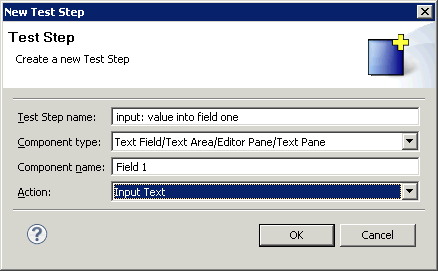
\includegraphics{Tasks/Teststeps/PS/teststepdialog}
\caption{New \gdstep{} Dialog}
\label{newstep}
\end{center}
\end{figure}

\textbf{Filling in the \gdstep{} dialog}\\
\textbf{\gdstep{} name}
\begin{enumerate}
\item In the \bxname{\gdstep Name} field, enter a name for the \gdstep{}. This name is just for recognition 
purposes, but should be easily identifiable at a later point. 

\textbf{Component type}
\item Select the component you want to test from the combo box. 

\bxtipp{A component is an element of the user interface you can execute an action on, e.g. a button, a text field.}

\textbf{Component name}
\label{componentnameteststep}
\item Enter a component name. This is your user-defined name that you will use to refer to this particular component. It will later be mapped to the real component in the \gdaut{}. Again, we suggest using conventions to name components \bxpref{BPComponentNames}. 

\item When you are entering component names, a combo box appears with a list of names you have already used. 

If any of the names are grayed out, this means they have been used for other component types and cannot be used for the currently selected component type. 

You can change, or \bxname{reassign} component names later when you reuse this \gdcase{}. Doing this means that you can execute the same actions on different components in the interface. The section on the \gdcompnamesview{} \bxpref{reass} contains information on reassigning component names. 

\textbf{Action}

\item From the combo box, choose the action you want to execute on this component. 
\bxtipp{Refer to the chapter on Components, Actions, and Parameters
(\bxextref{\jb{}efman}{ref,actparam}) for information on components, the
actions they support, and their parameters.}

\item Click \bxcaption{OK}. 
\item The \gdstep{} will appear as nested in the \gdcase{}.  
\bxtipp{You can change the position of \gdsteps{} using drag-and-drop.}

You can see and edit the details of any selected \gdstep{} in the \gdpropview{}.

The next step is to add parameter values (data) for \gdsteps{} in the \gdpropview{} \bxpref{WorkingWithData}. 
\end{enumerate}

%% \textbf{Concrete and abstract components in \gdsteps{}}
%% \label{teststepcomponent}
%% \begin{description}
%% \item[Concrete components]{ are components like \bxname{Combo Box} or \bxname{Text Field/Text Area/...} They refer to one single component or a few closely related components. Choosing a concrete component for a \gdstep{} restricts this \gdstep{} to this component. This isn't a problem if you are sure which component you will be testing.}
%% \item[Abstract components]{ are components like \bxname{Graphics Component} and \bxname{Button Component}. They are families of components, which all share similar features, and therefore similar action choices. Choosing an abstract component means that you have a larger choice of which real component  to test with this \gdstep{}. This is useful if you are at an early stage of development and are not exactly sure which component you will need to test. Choosing abstract components improves the  reusability of \gdcases{} because it makes the \gdcase{} more general and  flexible. It also makes the test easier to maintain because it increases the chance of being able to simply remap a changed component in the \gdaut{}. } 
%% \end{description}

%% If you have specified a specific toolkit or the \bxname{concrete} toolkit in the \gdaut{} configuration, you will be able to choose between abstract and concrete components. If you specified the \bxname{abstract} toolkit in the \gdaut{} configuration, you can only use abstract components. 


